\documentclass[handout]{beamer}

\title{Command Line Apps in Python}
\author{David Fischer}
\date{May 27, 2021}

%% Beamer Themes
\usetheme{Berlin}
\usecolortheme{dove}
\usefonttheme{serif}

%% Packages
% Pygments must be accessible to use minted and --shell-escape
%  must be used with pdflatex
\usepackage{minted}
\usepackage{hyperref}
\usepackage[font=scriptsize,labelformat=empty]{caption}


\setbeamertemplate{footline}{
  \hspace*{.2cm}
  \scriptsize{
    \insertshorttitle
    \hspace*{50pt}
    \hfill
    \insertframenumber/\inserttotalframenumber
    \hspace*{.2cm}
  }
  \vspace{9pt}
}


\begin{document}

\maketitle

\begin{frame}
\frametitle{}
  {\huge Why command line apps?}
\end{frame}


\begin{frame}
  \begin{itemize}
    \item Very flexible in terms of input and output
    \item Faster development time (and less maintenance)
    \item Easier to combine with other apps
  \end{itemize}
\end{frame}


\begin{frame}
  \begin{figure}[p]
    \centering
    \fbox{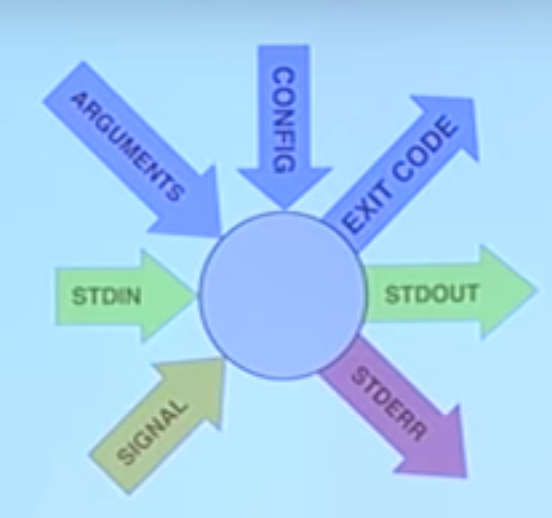
\includegraphics[height=0.7\paperheight]{includes/cli-inputs-outputs.png}}
    \caption{Borrowed from \href{http://pyvideo.org/europython-2014/writing-awesome-command-line-programs-in-python.html}{Mark Smith's 2014 Euro Python Talk}}
  \end{figure}
\end{frame}


% Fragile is required for syntax highlighting
\begin{frame}[fragile]
\frametitle{Argparse}

{\scriptsize
\begin{minted}{python}
## argparse_sample.py
import argparse
 
parser = argparse.ArgumentParser(description='This does almost nothing')
parser.add_argument('-v', '--version', 
                    action='version', version='%(prog)s 2.0')
args = parser.parse_args()
\end{minted}

\hfill

\begin{minted}{bash}
## Shell
$ python argparse_sample.py  -h
usage: argparse_sample.py [-h] [-v]
 
This does almost nothing
 
optional arguments:
  -h, --help     show this help message and exit
  -v, --version  show programs version number and exit
 
$ python argparse_sample.py  -v
argparse_sample.py 2.0
\end{minted}
}

\end{frame}


\begin{frame}[fragile]
\frametitle{Click}

{\scriptsize
\begin{minted}{python}
## click_sample.py
import click
@click.command()
@click.help_option('-h', '--help')
@click.version_option('2.0', '-v', '--version', message='%(prog)s v%(version)s')
def cli():
    """This does almost nothing"""
if __name__ == '__main__':
    cli()
\end{minted}

\hfill

\begin{minted}{bash}
## Shell
$ python click_sample.py  -h
Usage: click_sample.py [OPTIONS]

  This does almost nothing

Options:
  -h, --help     Show this message and exit.
  -v, --version  Show the version and exit.
$ python click_sample.py  -v
click_sample.py v2.0
\end{minted}
}

\end{frame}


\begin{frame}[fragile]
\frametitle{Click (continued)}

{\scriptsize
\begin{minted}{python}
import click
import os

plugin_folder = os.path.join(os.path.dirname(__file__), 'commands')

class MyMulticommand(click.MultiCommand):
    def list_commands(self, ctx):
        rv = []
        for filename in os.listdir(plugin_folder):
            if filename.endswith('.py'):
                rv.append(filename[:-3])
        rv.sort()
        return rv

    def get_command(self, ctx, name):
        ns = {}
        fn = os.path.join(plugin_folder, name + '.py')
        with open(fn) as f:
            code = compile(f.read(), fn, 'exec')
            eval(code, ns, ns)
        return ns['cli']
\end{minted}
}

\end{frame}



\begin{frame}
\frametitle{Resources}
  \begin{itemize}
    \item {\small A longer version of this talk is at \href{https://www.davidfischer.name}{davidfischer.name}}
    \item {\small Argparse tutorial: \href{https://docs.python.org/3.7/howto/argparse.html}{docs.python.org/3.7/howto/argparse.html}}
    \item {\small Click's documentation: \href{https://click.palletsprojects.com/}{click.palletsprojects.com}}
  \end{itemize}
\end{frame}


\begin{frame}
\frametitle{Future topics}
  \begin{itemize}
    \item {\small Packaging command line apps for distribution}
    \item {\small Testing command line apps}
    \item {\small Handling configuration and CLIs}
    \item {\small Structuring command line apps}
  \end{itemize}
\end{frame}


\end{document}
